% ==========================================================================
\chapter{Estimating the optimal port scanning technique}
\label{chapter:scanning-techniques-experiment}
% ==========================================================================

In this chapter, we present the results of three experiments that were conducted to estimate the most effective browser-based port scanning strategy for several combinations of operating system and browser. 
The first experiment focuses on estimating the optimal socket timeout setting, this experiment focuses on finding a balance between efficacy and efficiency.
The second experiment focuses on estimating the most effective scanning technique, this experiment focuses on the capability of JavaScript APIs to detect open ports.
The third experiment focuses on estimating the most efficient scanning technique, this experiment focuses on parallel connections.

\section{Definitions}

In order to address RQ1 effectively, it is crucial to establish clear definitions for attack goals, efficiency, and efficacy.

\subsubsection{Attack goals}

Attack goals refer to the specific objectives that an attacker aims to achieve by scanning ports. Generally, there are two common attack goals:

\begin{enumerate}[label=\alph*.]
    \item Enumerating the entire port range: This goal involves scanning all available ports on a target system to gather comprehensive information about its open and closed ports. It allows the attacker to obtain a broad understanding of the target's network services and potential vulnerabilities.
    
    \item Scanning for a specific number of ports: In this case, the attacker focuses on scanning a limited number of ports that are of particular interest. This targeted approach enables them to gather specific information related to those ports or services. It represents a trade-off between scanning for precise information and maximizing the amount of information gathered.
\end{enumerate}

It is worth noting that certain scanning techniques may be required to detect specific ports effectively, depending on the attack goals.

\subsubsection{Efficacy}

Efficacy is closely tied to the attack goal. 
It signifies the degree to which a scan successfully accomplishes its intended objective. 
The efficacy of a scan depends on whether the desired information can be obtained from one or more targeted ports.

For instance, if the attacker is scanning for a specific port, they may employ techniques tailored to detecting that port accurately. If the desired information can be retrieved from the scanned port(s), the scan is considered efficacious.

\subsubsection{Efficiency}

Efficiency is determined by various factors that impact the time and resources required to complete a scan. These factors include:

\begin{enumerate}[label=\alph*.]
    \item Number of parallel sockets: The number of parallel sockets running simultaneously during the scan affects how many ports can be scanned concurrently. Increasing the number of parallel sockets generally improves scan speed.
    
    \item Socket timeouts: Socket timeouts determine the duration for which the scanning tool waits for a response from each port. Optimal timeout settings balance the time required for accurate detection against minimizing delays.
    
    \item Number of scans to be executed: The number of scans an attacker intends to perform can impact efficiency. Performing multiple scans may be necessary to gather comprehensive information or increase the chances of successfully detecting specific ports.
    
    \item Additional overhead: Various factors such as browser, operating system, and hardware configurations can introduce overhead during the scanning process. These should be taken into account when evaluating efficiency.
\end{enumerate}

Efficiency is commonly assessed based on the time required to complete a scan. The faster a scan can be accomplished without compromising the desired efficacy, the more efficient it is considered. 


\section{Background}

This section provides an overview of potential scanning techniques that were considered for the experiment. Due to the constraints imposed by the abstraction layers provided by JavaScript APIs, the options are limited, every available JavaScript API capable of performing network requests was considered.

\subsection{Scanning techniques overview}
\subsubsection{Fetch API}

The Fetch API is a modern JavaScript API that provides an interface for making asynchronous HTTP requests. It allows us to send HTTP(S) requests to a specified URL and handle the responses. The Fetch API offers a more powerful and flexible alternative to the traditional XMLHttpRequest (XHR) approach.

\subsubsection{XMLHttpRequest (XHR)}

XMLHttpRequest is a JavaScript API that has been widely used for making asynchronous HTTP requests. It provides a way to send HTTP(S) requests to a server and receive responses. Although Fetch API is gaining popularity, XHR is still supported in most browsers and can be used for network requests.

\subsubsection{WebSocket}

WebSocket is a communication protocol that provides full-duplex communication channels over a single TCP connection. It enables real-time, bidirectional communication between a client and a server. WebSocket API in JavaScript allows establishing WebSocket connections and exchanging data between the client and the server.

% Below scanning techniques were considered, but deemed to be impossible to be used as a port scanning technique after conducting some experiments. These techniques can \emph{send} a stream of data over the network, but do not necessarily expect a response. It is therefore impossible to detect if a service might be running on a port using these scanning techniques.

\subsubsection{WebRTC}

WebRTC (Web Real-Time Communication) is a collection of communication protocols and APIs that enables peer-to-peer audio, video, and data sharing between browsers. It allows direct communication between browsers without the need for intermediate servers. WebRTC API provides methods to establish connections, exchange data, and control media streams.
WebRTC used to be a viable port scanning technique in the past, due to the \texttt{RTCPeerConnection.onicecandidateerror} event handler emitting useful error information about the status of the connection. However, after being exploited by Baines~\citearticle{baines2019} in 2019, 
this functionality has been removed for local connections~\citeartifact{webrtc}, and therefore scanning the local network via WebRTC is not possible anymore.

\subsubsection{Beacon API}

The Beacon API is a lightweight and efficient API for sending small amounts of data to a server asynchronously. It is designed for sending analytics data or other non-critical information without delaying or blocking the loading of the next page. The Beacon API is designed so that it can only \emph{send} data to a server, but not retrieve any. Therefore, we cannot use this API to determine the status of a port.

\subsubsection{Server-Sent Events}

Server-Sent Events (SSE) is a server push technology that enables continuous updates from the server to the client over a single HTTP(S) connection. However, SSE cannot be used for port scanning purposes due to its inherent design limitations. SSE operates on an event-driven model, where the server sends events to the client asynchronously. As SSE only allows data to flow from the server to the client and does not support client-initiated requests, it lacks the necessary functionality for conducting port scanning.

% ==========================================================================
\subsubsection{Scanning techniques comparison}
% ==========================================================================

The aforementioned JavaScript APIs leaves us with three possible APIs to perform browser-based port scanning: Fetch, XHR and WebSockets. As all three APIs are built on top of the TCP protocol, this limits the potential results that may be achieved, as the status of UDP ports will remain undetectable. 
While Fetch and XHR are similar in functionality, WebSockets are not built on top of the HTTP protocol, and could therefore achieve different results. WebSocket and HTTP are separate protocols that operate at layer 7 in the OSI model~\citescientific{kumar2014} and rely on TCP at layer 4. However, despite their differences, RFC 6455~\citetechnical{fette2011} specifies that WebSocket `is intended to be compatible with HTTP-based server-side software and intermediaries'. This compatibility is achieved through the WebSocket handshake, which utilizes the HTTP Upgrade header to transition from the HTTP protocol to the WebSocket protocol.
% This suggests that the WebSocket API could be the most effective scanning technique, as it is able to make requests over both the WebSocket and the HTTP protocol.

% ==========================================================================
\section{Experiment Setup}
% ==========================================================================

Having established the availability of three scanning techniques via the XHR, Fetch, and WebSocket APIs, we created an experiment to compare these techniques based on several metrics.

\subsection{Application design}
\label{section:port-scanner-application}

A client-side TypeScript web application was developed to facilitate a comparative analysis of these three JavaScript APIs. The application's design was guided by specific considerations outlined below, aimed at optimizing its functionality and applicability for forthcoming chapters.
Central to the application's design is the incorporation of configurability features. These features encompass essential parameters such as socket timeout, parallel socket connections, and the scanning technique. The rationale behind this emphasis on configurability lies in the necessity to ensure uniformity and consistency across various scans during the experiment. By maintaining consistent settings, the application enables accurate and meaningful comparisons between different scanning approaches.
These settings can be passed to the application using query parameters, as depicted in Figure~\ref{fig:initiate-scan}. 

\begin{figure}[ht]
    \centering
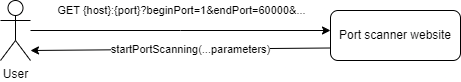
\includegraphics[width=10cm, height=10cm, keepaspectratio]{port_scanning_techniques/img/initiate_port_scan.png}
    \caption{User initiating port scan}
    \label{fig:initiate-scan}
\end{figure}

Upon requesting the webpage, a JavaScript file will be returned which initiates a scan on the localhost IP address. The available query parameters are listed in Table~\ref{tab:port-scan-params}. This solution was chosen to make the scans scriptable and therefore easily useable with automation frameworks such as Selenium.

\begin{table}[htbp]
\footnotesize
\centering
% \begin{adjustwidth}{-0.5cm}{}
\begin{tabular}{p{3cm} p{10cm}}
    \toprule
    Parameter & Description \\
    \midrule
    beginPort & The starting port for the scanning range. \\
    endPort & The final port for the scanning range. Scanning will be performed within the range from beginPort to endPort. \\
    nScans & The number of scan iterations for each individual port. For example, if nScans=10, each port within the specified range will be scanned 10 times. \\
    nSockets & The maximum number of sockets used for concurrent parallel scanning. \\
    socketTimeout & The time limit for a single scan attempt on a port. If the scan does not complete within this timeframe, the scanner aborts the scan and moves to the next port. \\
    scanningTechnique & The selected method for performing scans, such as fetch, xhr, or websockets. \\
    \bottomrule
\end{tabular}
% \end{adjustwidth}{}
\caption{Port scanner application available query parameters}
\label{tab:port-scan-params}
\end{table}

Existing client-side port scanning applications often share a common limitation known as batch-job scanning. In this approach, a predefined range of ports, such as ports 1-50, is scanned concurrently based on a configured parallel sockets count (referred to as "nSockets" in Table~\ref{tab:port-scan-params}). All ports within this designated range are scanned simultaneously within a batch. After completing the entire batch, the scanning process proceeds to the subsequent batch. However, this method suffers from inefficiencies due to variations in the time it takes to scan different ports. Consequently, there's a reduced number of parallel sockets, typically less than 50, actively operating at any given time. This limitation hampers the overall efficiency of the scanning process.
To overcome this limitation, we have created a queuing mechanism designed to eliminate this limitation and ensure optimal utilization of parallel sockets throughout the scanning process. This queuing system operates on the principle of promptly dequeuing a scanning job once the scan of a port is completed. By adopting this approach, our application guarantees a consistent and maximum utilization of parallel sockets throughout the entire scanning operation. This queuing mechanism optimally distributes scanning tasks, minimizing idle periods, and thereby significantly enhancing the efficiency of the scanning process.

This improvement is illustrated by comparing the two techniques in Figures~\ref{fig:batch-job} and~\ref{fig:queue-job}. The comparison visually demonstrates port scans on six ports, with three scans concurrently executed in parallel. In this hypothetical scenario, a reduction of 100ms in scanning time is simulated. While this incremental gain might seem minor when scanning a limited number of ports, say 1000, its impact becomes notably significant when extending the scope of the scan to encompass the entire port range, spanning from 0 to 65536.

\begin{figure}[htbp]
    \centering
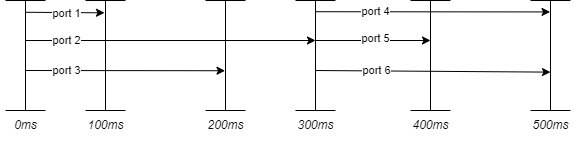
\includegraphics[width=10cm, height=10cm, keepaspectratio]{port_scanning_techniques/img/batch-job.jpg}
    \caption{Batch-job scanning}
    \label{fig:batch-job}
\end{figure}

\begin{figure}[htbp]
    \centering
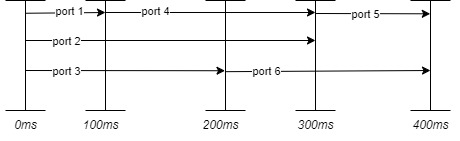
\includegraphics[width=10cm, height=10cm, keepaspectratio]{port_scanning_techniques/img/queue-job.jpg}
    \caption{Queueing jobs concurrently}
    \label{fig:queue-job}
\end{figure}

By adopting the queuing mechanism, our approach mitigates the inefficiencies inherent in batch-job scanning, leading to a substantial improvement in the efficiency and speed of port scanning, particularly when dealing with a larger range of ports.
When all ports have finished scanning, the results of the scan are posted back to the server for post-scan analysis. The implementation of the full application can be found on GitHub~\citeartifact{bvdl2023}

\subsection{Docker Containerization}
\label{section:experiment-setup}

In order to conduct our experiments systematically and ensure reproducibility, we employed a fully automated approach utilizing Docker containers. 
This approach encapsulated the entire experiment, maintaining consistency and facilitating the ability to replicate the experiments precisely. 
The setup was designed to be repeatable by others.

We employed Docker containers to establish a self-contained and isolated environment for conducting our experiments. This approach effectively eliminated potential issues that could arise from variations in the underlying host systems.
The use of Docker containers provided us with the capability to define and manage various experiment parameters, including operating systems, web browsers, socket settings, and scanning techniques, all through Dockerfiles. This ensured that the experiment environment remained consistent and reproducible across multiple runs.

Within these Docker containers, we included servers that served as potential attack targets. Among them, there is a server that hosts an implementation of the browser-based port scanning application, simulating a website running browser-based port scanning attacks. Furthermore, our Docker containers also contain a client-side Selenium application responsible for initiating and interacting with the browser-based port scanning application during the experiments, utilizing headless browsers.

\subsubsection{Automated Scripting}

We developed automated scripts to orchestrate and execute the experiments within the Docker containers. These scripts facilitated the setup and execution of the scans, with precise control over the scanning parameters.
The automation enabled us to easily run multiple experiments in a scripted manner, ensuring accurate and reproducible results.

\subsubsection{Data Collection Metrics}

Throughout the experiments, we systematically gathered data with a focus on two key metrics: efficacy and efficiency.

\begin{itemize}
    \item \textbf{Efficacy} was defined by the count of accurately identified open ports.
    \item \textbf{Efficiency} was evaluated by analyzing the speed of the scanning process while ensuring that the efficacy of port detection remained uncompromised.
    \item For each scan, we collected the following metrics:
    \begin{itemize}
        \item A timestamp indicating when the scan started and ended.
        \item The port number and its status (open/closed).
        \item Start and end times of each individual port scanned.
    \end{itemize}
    \item Additionally, post-scan analysis was employed to determine port status via timing measurements.
\end{itemize}

\subsubsection{Experiment Reproducibility}
\begin{itemize}
    \item To ensure the reproducibility of the experiments, we shared Docker images and scripts used for the experiments, allowing other researchers to replicate our setup easily.
    \item The encapsulation and isolation provided by Docker containers guaranteed a consistent experiment environment, irrespective of the host system's variations.
\end{itemize}

The utilization of Docker containers for our experiments effectively addressed the challenges related to reproducibility in scientific research. The experimental setup is visually represented in Figure~\ref{fig:experiment}.

\begin{figure}[tbh]
    \centering
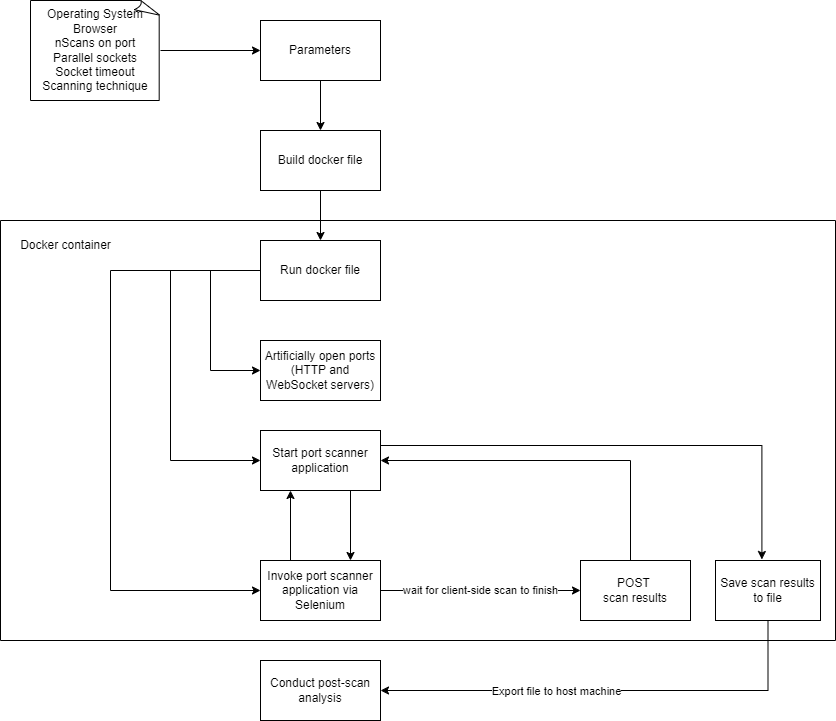
\includegraphics[width=15cm, height=15cm, keepaspectratio]{port_scanning_techniques/img/portscan_experiment.png}
    \caption{Experiment setup}
    \label{fig:experiment}
\end{figure}


% Besides this queueing mechanism, we implemented an abstraction layer which enables us to pass a different scanning function (XHR, Fetch, WebSocket) without having to make functional changes to the underlying logic. The only difference in logic is the scanning technique implementation. The implementation of the port scanner application can be found on GitHub~\cite{bvdl2023}

% \section{Experiments}

% Three experiments were conducted to estimate the optimal browser-based port scanning. The overarching objective of these experiments was to discern the most suitable port scanning technique for each unique combination of operating system and browser. This discernment serves as a foundation for subsequent chapters, wherein deeper exploration into the capabilities of browser-based port scanning is undertaken.

\section{Experiment 1: Estimating the optimal socket timeout setting}
\label{section:socket-timeout-setting}

In the context of browser-based port scanning, there are two key motivations for considering the adjustment of the socket timeout setting:
\subsection{Motivation}
\subsubsection{Enhancing Scan Efficiency}

One primary motivation for altering the socket timeout setting is to improve the efficiency of the port scanning process. This involves two key aspects:

\begin{itemize}
  \item \textbf{Faster Scanning}: By lowering the socket timeout, the scanner spends less time waiting for responses from each port. Consequently, this leads to quicker scans, as the scanner can move on to the next port faster.

  \item \textbf{Efficiency Gains}: Ultimately, the objective is to achieve higher overall efficiency, enabling the scanning of more ports within a shorter time frame. This is particularly important when conducting large-scale or time-sensitive scans.
\end{itemize}

\subsubsection{Balancing Efficacy and Speed}

While efficiency gains are desirable, there is an inherent trade-off between scan speed and efficacy when adjusting the socket timeout setting:

\begin{itemize}
  \item \textbf{Efficacy Concerns}: Setting the socket timeout too low might result in inaccurate scan results. In such cases, the scanner may not wait long enough to receive a response from the target port, potentially leading to false negatives.

  \item \textbf{Finding the Optimal Balance}: Therefore, it becomes crucial to strike a balance between efficacy and efficiency. The challenge lies in identifying the lowest socket timeout value that maintains efficacy without sacrificing scan efficiency.
\end{itemize}

\subsection{Experiment Target}

In order to address the motivations outlined above, the experiment targets the following objectives:

\subsubsection{Determining the Optimal Socket Timeout}

\begin{itemize}
  \item \textbf{Objective}: The primary objective of the experiment is to identify the socket timeout value that strikes the ideal balance between scan speed and efficacy.
  
  \item \textbf{Analysis of Results}: Data collected during the experiment is analyzed comprehensively to determine which socket timeout setting achieves this balance most effectively.
  
  \item \textbf{Validation}: The identified optimal socket timeout value is further validated by conducting additional scans on different target systems. This validation step ensures that the selected setting is applicable and reliable across various scanning scenarios, providing a robust solution for future port scanning endeavors.
\end{itemize}

\subsubsection{Socket Timeout Adjustment}

\begin{itemize}
  \item \textbf{Socket Timeout Setting}: The primary variable under investigation in this experiment is the socket timeout setting.
  
  \item \textbf{Range of Values}: The experiment involves testing a range of socket timeout values, spanning from very low settings to moderate values.
  
  \item \textbf{Measurement of Efficiency}: Efficiency in this context is quantified by measuring the time taken to complete the port scan for each tested socket timeout value.
  
  \item \textbf{Measurement of Efficacy}: To assess efficacy, the scan results are compared against a reference set of known open and closed ports.
\end{itemize}

The parameters for the experiments can be found in Appendix~\ref{appendix:expirement-parameters}. 
We chose not to include MacOS in the list of Operating Systems because of compatibility issues with Docker.


% \subsection{Experiment Setup}

% The automated setup as outlined in Section~\ref{section:experiment-setup} was used for the experiment. Several Docker images were created using different operating systems, browsers, and socket timeout settings. These parameters are listed in Appendix~\ref{appendix:expirement-parameters}.

\subsection{Experiment Results}

In this experiment, we investigated the impact of varying socket timeout settings on the efficacy and efficiency of port scanning using different web browsers and operating systems. The key findings are summarized below:

\subsubsection{Socket Timeout Settings and Efficacy}

We observed that the choice of socket timeout setting significantly affected the efficacy of port scanning, particularly for the Chrome and Firefox browsers. Specifically:

\begin{itemize}
    \item \textbf{Chrome Browser}:
    \begin{itemize}
        \item Using a socket timeout of 100 milliseconds resulted in reduced efficacy, with 76 ports being detected rather than the configured 100 open ports.
        \item The efficacy reached 100\% when a socket timeout setting of 150ms was used.
    \end{itemize}
    
    \item \textbf{Firefox Browser}:
    \begin{itemize}
        \item Similar outcomes were measured for Firefox, with a timeout of 100 milliseconds resulting in only 21 detected ports.
        \item The efficacy reached 100\% when a socket timeout setting of 150ms was used.
    \end{itemize}
\end{itemize}

The raw results can be found in Appendix A, Table~\ref{tab:socket-timeout-comparison}.

\subsubsection{Real-world Validation}

To ensure the reliability of our findings, we conducted real-world validation of the results obtained within our virtualized environment. The validation process revealed interesting insights:

\begin{itemize}
    \item \textbf{Chrome's Consistency}: After validating the results in a real-world scenario, Chrome's efficacy remained consistent at 100\% with a 150ms timeout, reinforcing the reliability of this setting.
    
    \item \textbf{Firefox's Variable Performance}: In contrast, Firefox's results were inconsistent until a timeout of 400ms was used in a real-world context. This variability highlights the importance of considering real-world scenarios in setting optimal socket timeouts.
\end{itemize}


\subsubsection{Socket Timeout Behavior in Different Operating Systems}
\label{section:socket-timeout-comparison}

In our experiments, we observed a notable difference in how socket timeout settings are handled by different operating systems.

\begin{itemize}
    \item \textbf{Windows Operating System}:
    \begin{itemize}
        \item Windows respects the configured socket timeout setting as defined in the scanning parameters.
        \item The efficacy and timing of port responses closely align with the specified timeout, making the socket timeout setting a critical factor in scan efficacy and efficiency on Windows.
    \end{itemize}
    
    \item \textbf{Ubuntu Operating System}:
    \begin{itemize}
        \item In contrast, Ubuntu exhibits a distinct behavior. The operating system ignores the configured timeout and automatically times out the request when possible.
        \item Ports generally respond within a range of 5--75 milliseconds on Ubuntu, irrespective of the configured socket timeout setting.
        \item This behavior makes socket timeout settings less critical on Ubuntu, as the automatic request timeout mechanism often results in responses occurring well within the specified timeout.
    \end{itemize}
\end{itemize}


\subsection{Analysis}

The socket timeout settings play a pivotal role in determining the efficacy and efficiency of browser-based port scanning.

\begin{enumerate}
    \item \textbf{Chrome Browser}: A socket timeout setting of 150ms consistently achieves 100\% efficacy in both virtualized and real-world environments. It strikes an optimal balance between efficacy and speed for Chrome.
    \item \textbf{Firefox Browser}: A longer timeout of 400ms is advised for Firefox, as we measured that the optimal socket timeout of 150ms during our testing was not accurate during real-world validation. This difference can be attributed to the headless Firefox browser used in our experiments, which is considerably more efficient than the regular browser used in real-world scanning scenarios.
    \item \textbf{Ubuntu Operating System}: Ubuntu's automatic request timeout mechanism minimizes the influence of socket timeout settings. Responses generally occur within 5-75ms, making precise tuning of the socket timeout setting less critical. 
    \item \textbf{Windows Operating System}: On Windows, socket timeout settings have a more pronounced impact. The operating system respects the configured socket timeout setting, leading to a loss of efficacy in the scan results when the socket timeout is too low. 
\end{enumerate}

\subsubsection{Conclusion}

In the context of browser-based port scanning, adjusting the socket timeout setting serves two key purposes:

\begin{enumerate}
    \item \textbf{Efficiency Improvement}: Lowering the socket timeout accelerates scanning, enhancing efficiency for large-scale or time-sensitive scans.
    \item \textbf{Balance between Efficacy and Efficiency}: Striking the right balance between efficacy and efficiency is crucial. An overly low timeout compromises efficacy, while a very high timeout compromises efficiency.
\end{enumerate}

Our experiments recommend a socket timeout of 150ms for Chrome and 400ms for Firefox. These settings ensure efficient scans on both Windows and Ubuntu while maintaining a 100\% detection rate of open ports. It is worth noting that Ubuntu's automatic request timeout mechanism minimizes the influence of socket timeout settings, making precise tuning less critical on this operating system.

\section{Experiment 2: Estimating the most effective scanning technique}

\subsection{Motivation}

\begin{itemize}
    \item \textbf{Efficacy}: The motivation behind this experiment is to identify the most effective scanning technique for browser-based port scanning.
    \item \textbf{Comparing scanning techniques}: The goal is to determine which of the three scanning technique -- Fetch, XHR (XMLHttpRequest), and WebSocket APIs -- offers the highest efficacy in detecting open ports.
\end{itemize}

\subsection{Experiment Target}

The experiment is designed to investigate and compare the efficacy of different scanning techniques, namely the Fetch, XHR and WebSocket APIs.

The experiment targets the following specific objectives:
\begin{itemize}
    \item Evaluate the efficacy of each scanning technique in detecting open ports using the intended functionality of the APIs.
    \item Evaluate the efficacy of each scanning technique in detecting open ports using a timing attack method.
\end{itemize}


% \subsection{Experiment Setup}

% The automated setup as outlined in Section~\ref{section:experiment-setup} was used for the experiment. Several Docker images were created using different operating systems, browsers, and different attack targets (servers representing attack objectives), These parameters are listed in Appendix A~\ref{appendix:experiment-parameters}.

\subsection{Experiment Results}

In this experiment, we evaluated the efficacy of three scanning techniques –- the Fetch, XHR, and WebSocket APIs –- with the optimal socket timeout setting determined in the previous experiment. The raw results can be found in Table~\ref{tab:scan-technique-comparison}.

\subsubsection{Fetch API Outperforms}

\begin{itemize}
    \item The Fetch API demonstrated superior performance, achieving a 100\% open port detection rate.
    \item This success can be attributed to its unique ability to operate in the \emph{no-cors} mode within JavaScript, allowing cross-domain requests, including requests to localhost, without CORS restrictions.
\end{itemize}

\subsubsection{XHR and WebSocket with Post-Scan Analysis}

\begin{itemize}
    \item Initially, both the XHR and the WebSocket APIs struggled to detect open ports and exhibited a 0\% detection rate using the intended functionality of the respective APIs.
    \item However, post-scan analysis revealed their potential by comparing response times between closed and open ports. Ports responding within less time than the configured socket timeout were consistently found to be open on the Windows operating system.
    \item The timing attack method was not applicable on the Ubuntu operating system due to response times being similar between open and closed ports.
\end{itemize}

Particularly on the Windows operating system, the XHR and WebSocket  detection capabilities were significantly enhanced when utilizing this timing attack method, enabling the XHR API to achieve a 100\% open port detection rate. This is depicted in Figures~\ref{fig:win-chrome-xhr} and~\ref{fig:win-firefox-xhr}.

\begin{figure}[ht]
\centering
\begin{minipage}{.45\textwidth}
  \centering
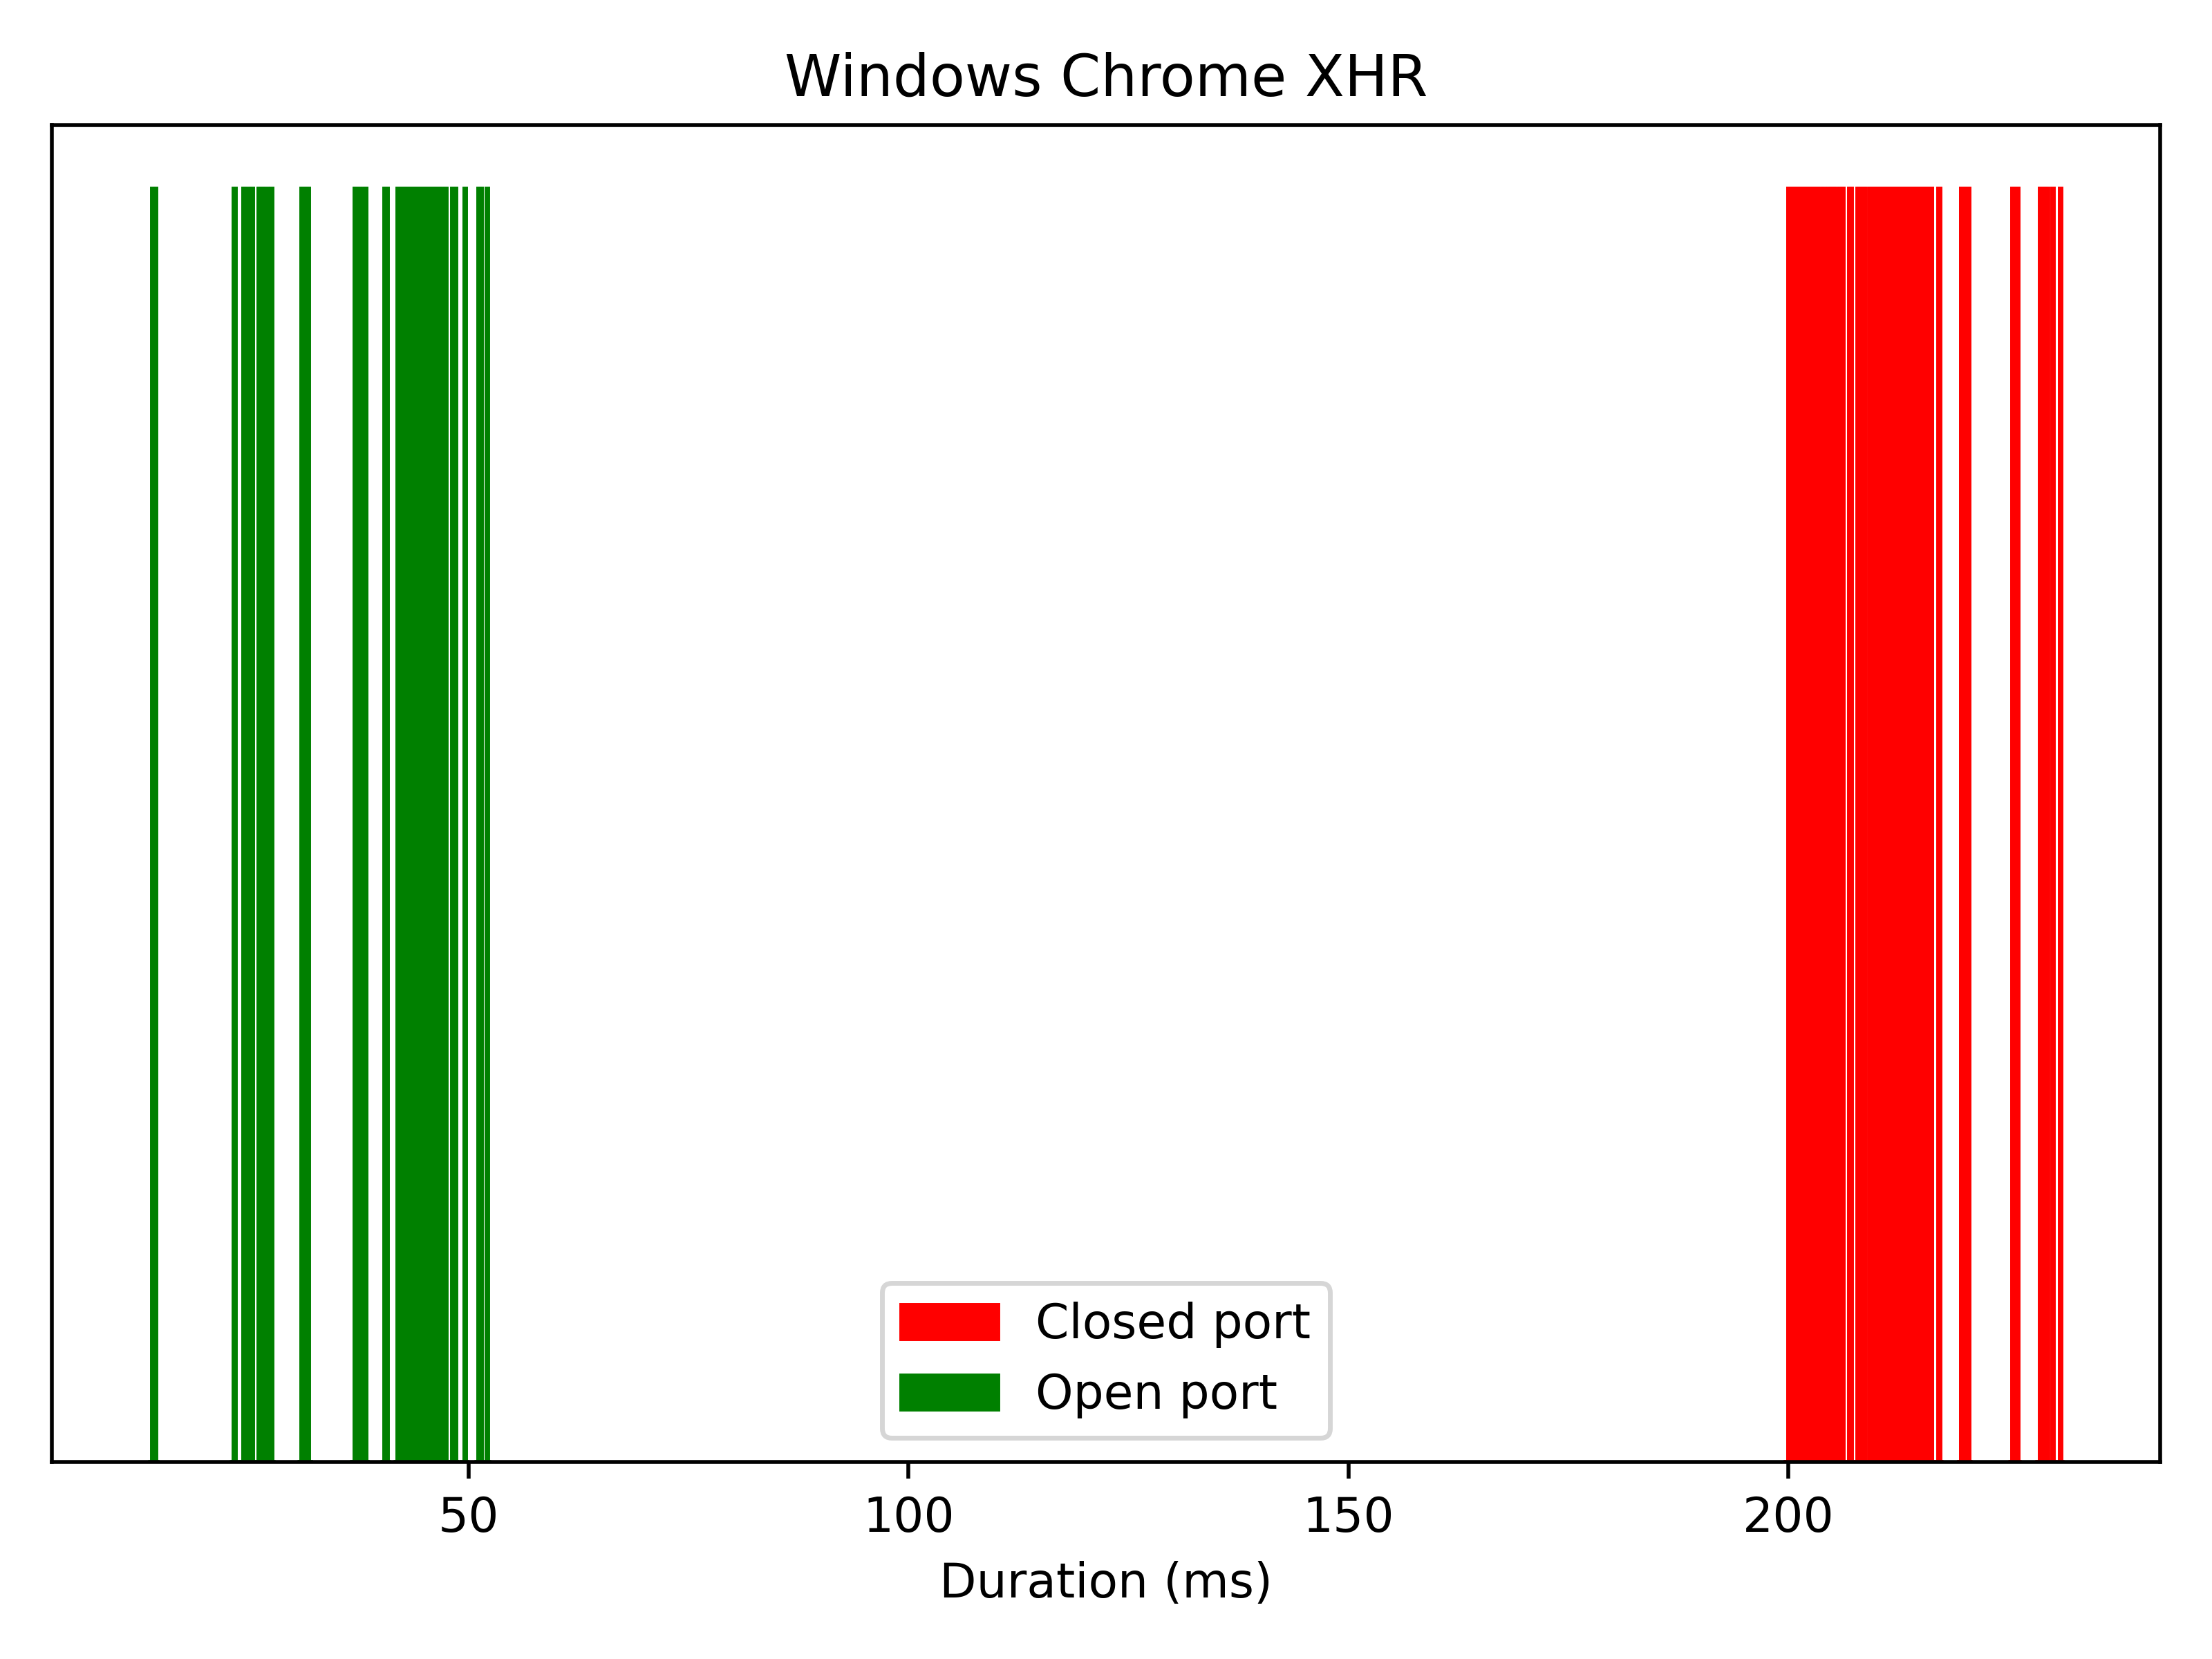
\includegraphics[width=10cm, height=5cm, keepaspectratio]{port_scanning_techniques/img/windows_chrome_efficacy_xhr.png}
    \caption{Windows/Chrome XHR API scan duration open vs closed ports}
    \label{fig:win-chrome-xhr}
\end{minipage}
\hspace{0.5cm} % Adjust the horizontal space between the two figures
\begin{minipage}{.45\textwidth}
\includegraphics[width=10cm, height=5cm, keepaspectratio]{port_scanning_techniques/img/windows_firefox_efficacy_xhr.png}
    \caption{Windows/Firefox XHR API scan duration open vs closed ports}
    \label{fig:win-firefox-xhr}
\end{minipage}
\end{figure}

The combination of WebSocket/Firefox also had an increased detection rate of 100\%, but WebSocket/Chrome remained unable to detect any of the open ports, this is depicted in Figures~\ref{fig:win-firefox-websocket} and~\ref{fig:win-chrome-websocket}. Further comparisons can be found in Appendix A, Section~\ref{appendix:scan-duration-comparison}

\begin{figure}[ht]
\centering
\begin{minipage}{.45\textwidth}
  \centering
\includegraphics[width=8cm, height=4cm, keepaspectratio]{port_scanning_techniques/img/windows_Firefox_efficacy_websocket.png}
    \caption{Windows/Firefox WebSocket API scan duration open vs closed ports}
    \label{fig:win-firefox-websocket}
\end{minipage}
\hspace{0.5cm} % Adjust the horizontal space between the two figures
\begin{minipage}{.45\textwidth}
  \centering
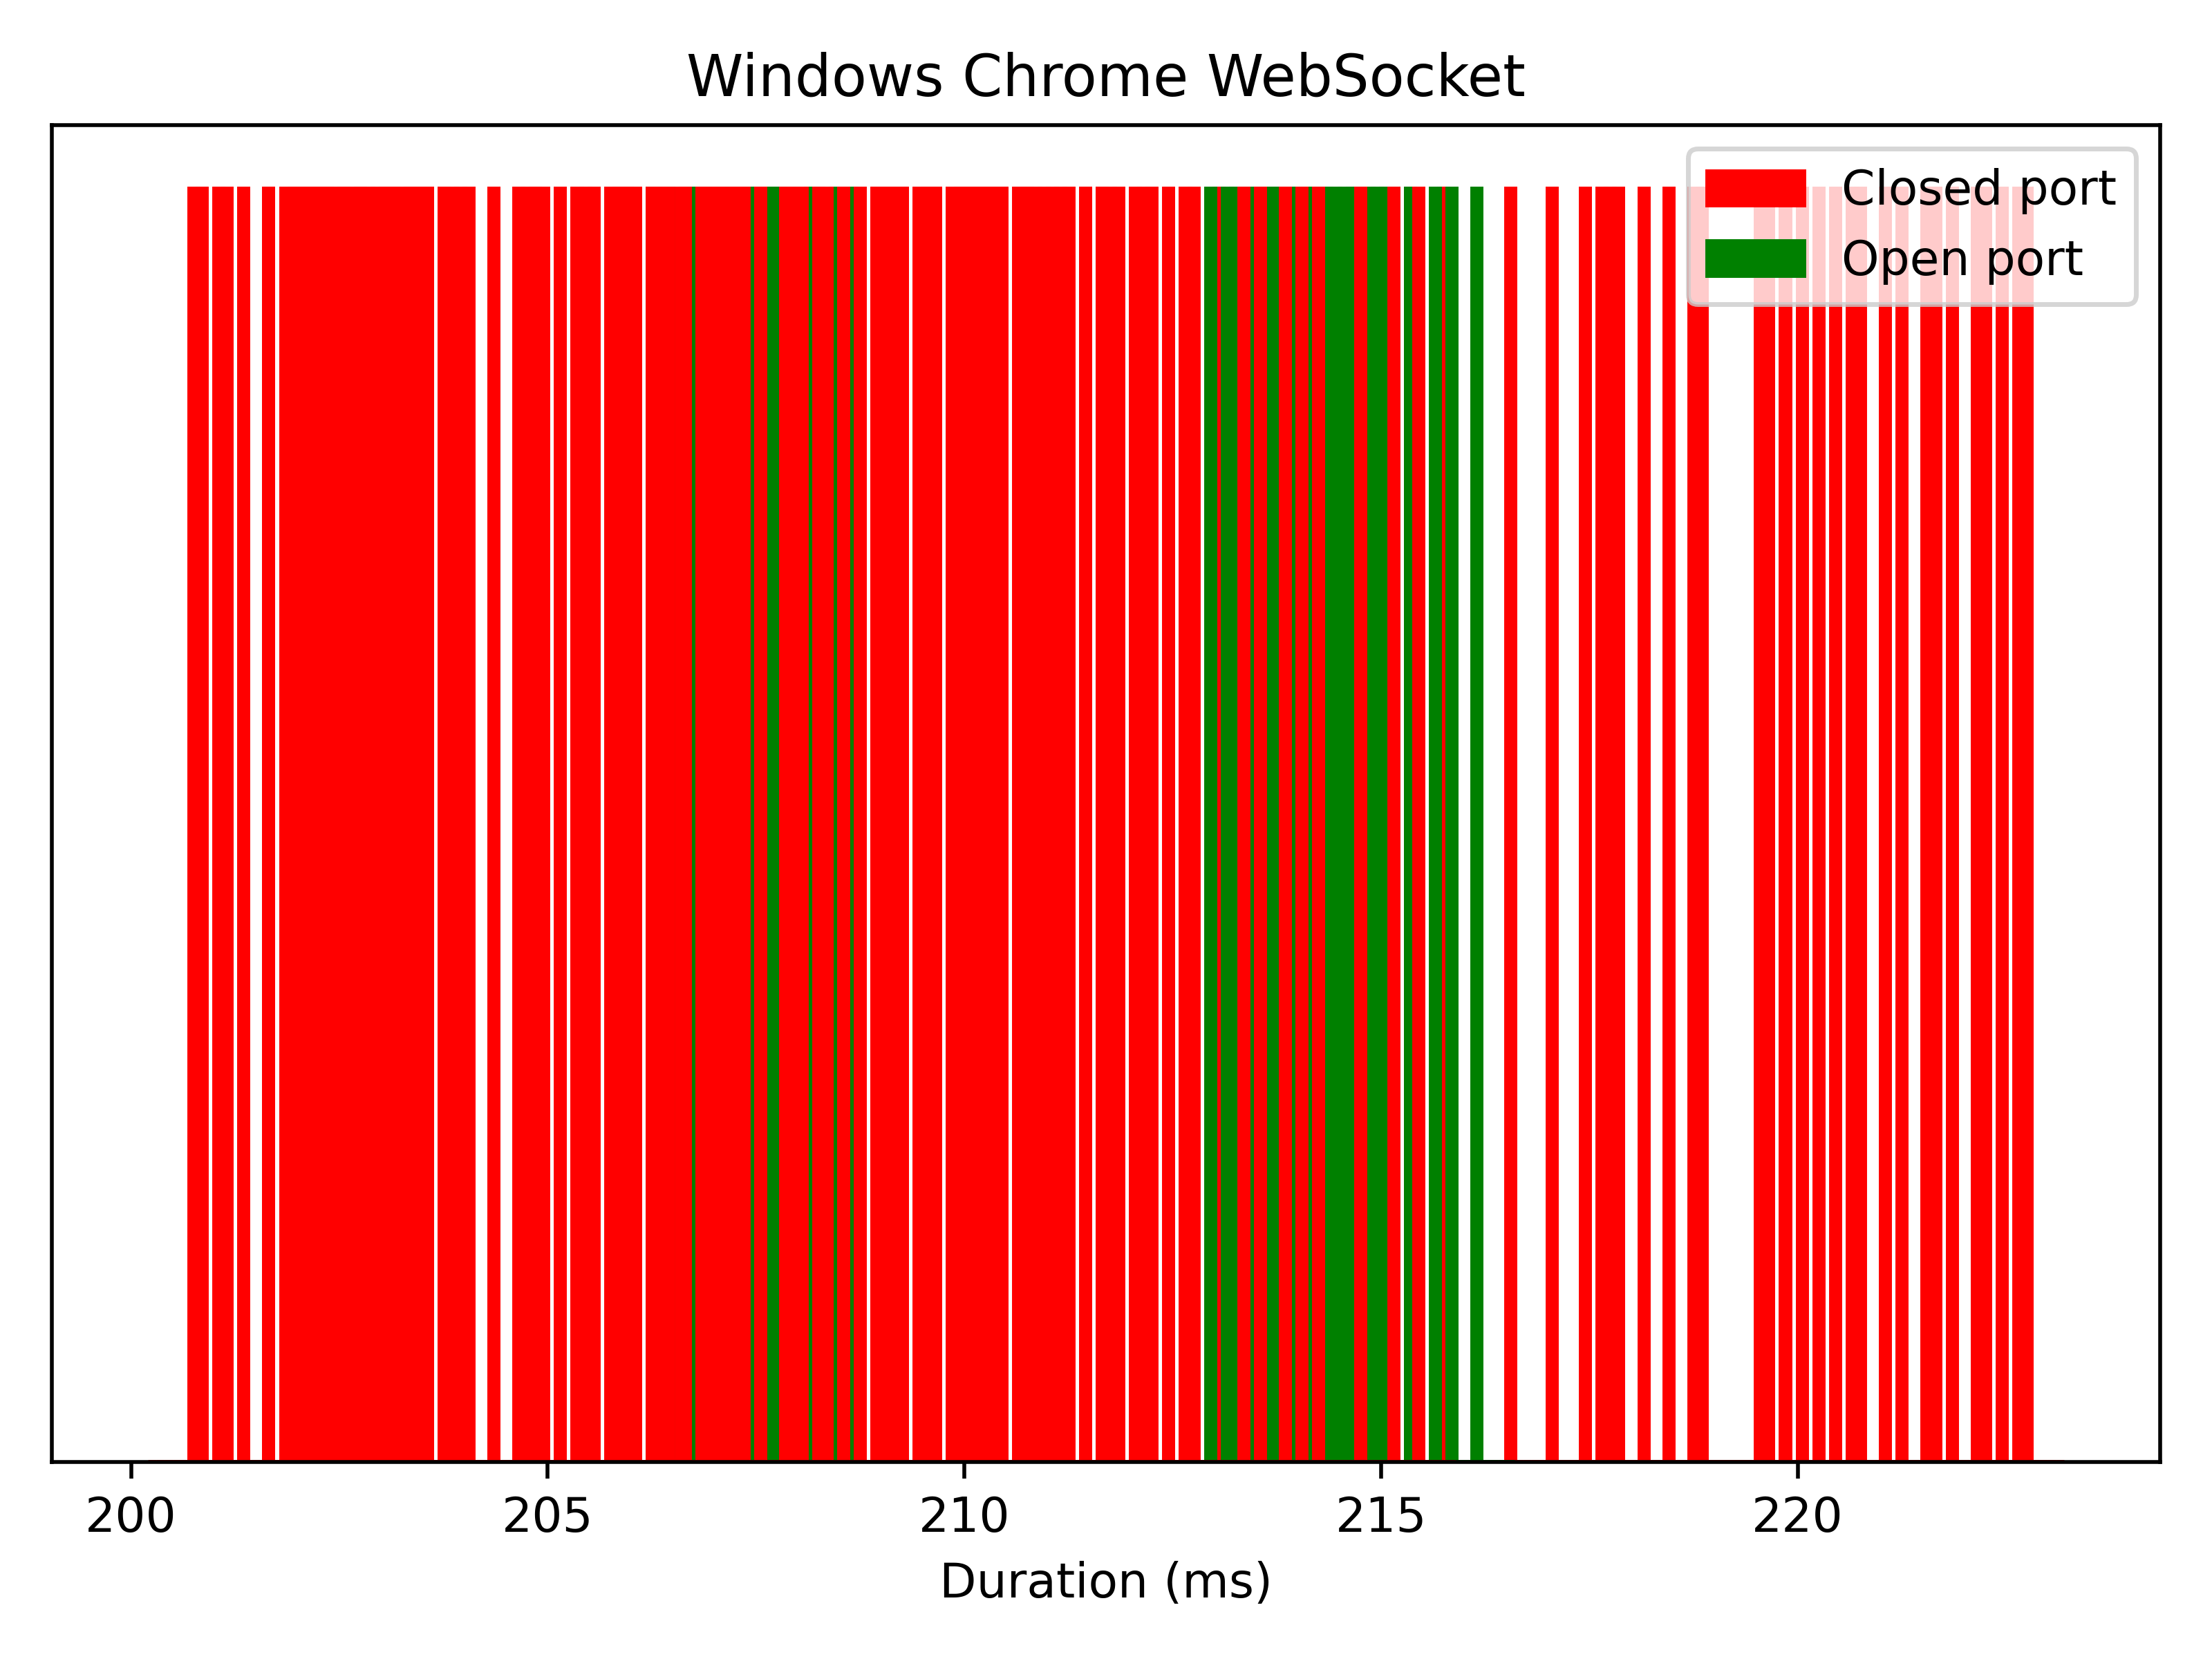
\includegraphics[width=8cm, height=4cm, keepaspectratio]{port_scanning_techniques/img/windows_chrome_efficacy_websocket.png}
    \caption{Windows/Chrome WebSocket API scan duration open vs closed ports}
    \label{fig:win-chrome-websocket}
\end{minipage}
\end{figure}

\subsection{Analysis}

\subsubsection{Fetch API Advantage}

\begin{itemize}
    \item The Fetch API's success lies in its \emph{no-cors} mode, allowing it to bypass CORS restrictions and reliably detect open ports.
    \item Despite limitations in this mode, such as restricted headers and inability to access response details, the Fetch API is able to reliably determine open HTTP ports using this method.
\end{itemize}


\subsubsection{XHR and WebSocket Potential}

\begin{itemize}
    \item While XHR and WebSocket APIs initially struggled to detect any open ports using their native API functionality, however, post-scan analysis utilizing response time measurements unveiled their potential.
    \item The timing attack method significantly enhanced their performance on Windows systems, achieving a 100\% open port detection rate.
    \item However, the absence of a clear response time distinction between open and closed ports on Ubuntu limits the applicability of this method.
\end{itemize}

\subsubsection{Consideration of Unsafe Ports}

The presence of \emph{unsafe} ports~\citetechnical{firefox_restricted_ports}\citeartifact{chrome_restricted_ports}, which cannot be reliably classified as open or closed, introduces complexity to port scanning.
Unsafe or restricted ports refer to a range of TCP/UDP ports that are reserved for system or administrative use and are not meant for normal application traffic. Browsers do not reveal information about these ports, so we cannot determine whether these ports are open or not. Unsafe ports were excluded from the results to prevent data pollution.


\subsubsection{Conclusion}

The motivation behind this experiment was to identify the most effective scanning technique for browser-based port scanning. We aimed to determine which of the three scanning techniques -- Fetch API, XHR, and WebSocket API -- offers the highest efficacy in detecting open ports.

Based on our analysis, it is evident that the Fetch API excels across all platforms (OS/Browser combinations) and stands as the superior choice for browser-based port scanning. 
This API enables us to scan for open ports and directly determine their status, eliminating the need for post-scan analysis or the use of timing attacks when scanning for ports running HTTP.


\section{Experiment 3: Estimating the most efficient scanning technique}

\subsection{Motivation}

\begin{itemize}
    \item \textbf{Efficiency}: This experiment focuses on optimizing the efficiency of port scanning. The primary aim is to explore how varying the number of parallel connections impacts scanning efficiency when scanning the entire port range (0-65536). 
    \item \textbf{Identifying the potential of a real world attack}: Without measuring efficiency, it is unclear how realistic a real world attack is, and how many ports can be scanned in practice.
\end{itemize}

\subsection{Experiment Target}

This experiment targets specific objectives related to efficiency and parallel connections:

\begin{itemize}
    \item \textbf{Evaluate Scanning Technique Efficiency}: Assess the efficiency of different scanning techniques when scanning the entire port range (0-65536).
    \item \textbf{Study the Impact of Parallel Connections}: Investigate how the number of parallel connections affects the scanning process.
    \item \textbf{Find Optimal Parallel Connections}: Identify the optimal number of parallel connections that maximizes scanning efficiency.
\end{itemize}

% \subsection{Experiment Setup}

% The automated setup as outlined in Section~\ref{section:experiment-setup} was used for the experiment. Several Docker images were created using different operating systems, browsers, and different number of parallel connections, These parameters are listed in Appendix A~\ref{appendix:experiment-parameters}.

\subsection{Experiment Results}

\begin{itemize}
  \item \textbf{Ubuntu vs. Windows:} Notable distinctions were observed between Ubuntu and Windows in terms of scanning efficiency using Fetch and XHR APIs. Ubuntu exhibited superior performance compared to Windows, which was partly attributed to Ubuntu's disregard for the configured socket timeout.

  \item \textbf{Parallel Connections on Ubuntu:} Increasing the number of parallel connections on Ubuntu did not provide significant performance benefits. Efficiency gains were marginal, and performance even slightly decreased with a larger number of connections. A configuration of around 10 parallel connections demonstrated the highest efficiency.

  \item \textbf{The most effective scanning techniques:} The three APIs exhibited similar behavior on Windows. On Ubuntu, the XHR and Fetch APIs significantly outperformed the WebSocket API.
  
  Ubuntu's behavior aligned with that of Windows when WebSockets were used. Fetch and XHR connections completed significantly faster on Ubuntu compared to WebSockets.

  \item \textbf{Scanning Time:} Ubuntu completed scanning the entire port range within 25 seconds, while Windows took 50 seconds even with the highest number of parallel connections (250).

\end{itemize}

These findings, illustrated in Figures~\ref{fig:windows_chrome_n_sockets} and~\ref{fig:ubuntu_chrome_n_sockets}, provide insights into the optimal scanning techniques for different operating systems and the impact of parallel connections on scanning efficiency. Further comparisons can be found in Appendix A, Section~\ref{appendix:efficiency-comparison}

\begin{figure}[ht]
\begin{adjustwidth}{-2cm}{-1cm}
\centering
\begin{minipage}{.45\textwidth}
  \centering
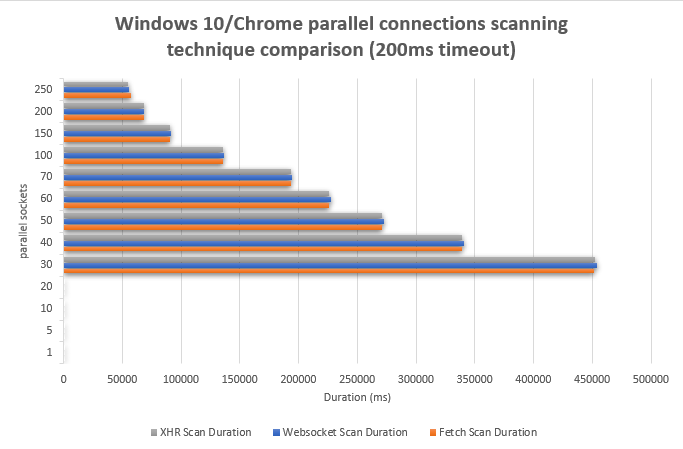
\includegraphics[width=10cm, height=7cm, keepaspectratio]{port_scanning_techniques/img/windows_chrome_scan_technique_comparison.png}
    \caption{Windows/Chrome Parallel sockets efficiency comparison}
    \label{fig:windows_chrome_n_sockets}
\end{minipage}
\hspace{2.6cm}
\begin{minipage}{.45\textwidth}
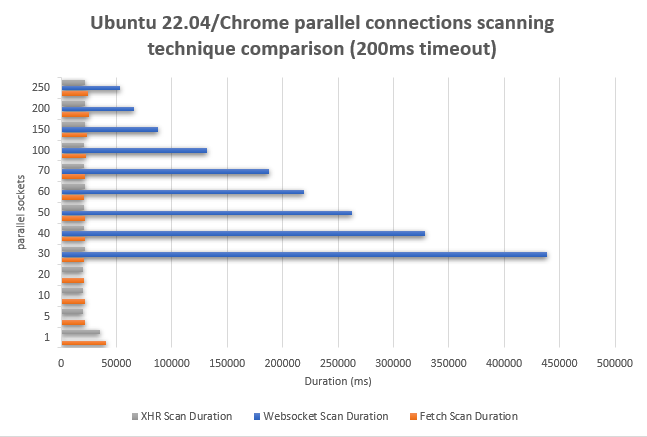
\includegraphics[width=10cm, height=7cm, keepaspectratio]{port_scanning_techniques/img/ubuntu_chrome_scan_technique_comparison.png}
    \caption{Ubuntu/Chrome Parallel sockets efficiency comparison}
    \label{fig:ubuntu_chrome_n_sockets}
\end{minipage}
\end{adjustwidth}
\end{figure}


\subsection{Analysis}

\begin{itemize}

\item \textbf{Optimal number of parallel connections:} We estimate the optimal number of parallel connections to be roughly 10 on Ubuntu, and as high as possible on Windows (250 during our testing). This distinction stems from the fact that Ubuntu does not respect the configured socket timeout, as described in Section~\ref{section:socket-timeout-comparison}. Windows does respect this timeout setting, and is therefore more efficient the more connections it can use. However, when increasing the number of parallel connections on Ubuntu, the socket timeout slowly increases, making the usage of more concurrent connections less efficient. For that reason, it is vital to strike a balance on Ubuntu, which we found to be roughly 10 concurrent connections. 
\item \textbf{Practical Considerations:} Using an excessively high number of parallel connections may seem beneficial in theory (i.e. 200+ parallel connections on Windows) but introduces severe delays and renders the webpage unusable for the user. This practical consideration underscores the irrelevance of establishing a theoretical limit for parallel connections in real-world scenarios.

\end{itemize}

\subsubsection{Conclusion}

The motivation behind this experiment was twofold. Firstly, we aimed to optimize the efficiency of port scanning, focusing on the impact of varying the number of parallel connections when scanning the entire port range (0-65536). Secondly, we sought to identify the potential of a real-world attack by measuring scanning efficiency, providing insights into the feasibility of such attacks.

The experiments have yielded the following findings:

\begin{itemize}
    \item \textbf{Ubuntu vs. Windows Efficiency}: Notable distinctions were observed between Ubuntu and Windows in terms of scanning efficiency. Ubuntu efficiently scanned the entire port range within 25 seconds, whereas Windows took 50 seconds, even with the highest number of parallel connections (250).

    \item \textbf{Balancing Parallel Connections and Timeouts}: Achieving optimal efficiency in port scanning involves striking a balance between the number of parallel connections and socket timeouts. Ubuntu's expedited socket timeouts were closely related to the number of parallel connections, with the most efficient setting observed at approximately 10 parallel connections.

    \item \textbf{Practicality in Real-World Attacks}: Although using a high number of parallel connections may seem theoretically advantageous, it introduces significant delays and renders webpages unusable for users. Therefore, establishing a theoretical limit for parallel connections, such as increasing the count to 256 instead of 250, was deemed irrelevant. In practice, both amounts are impractical for real-world port scan attacks on Windows.

\end{itemize}

In conclusion, this experiment has provided valuable insights into optimizing the efficiency of port scanning techniques. It has demonstrated that the efficiency of port scanning varies significantly between Ubuntu and Windows, with Ubuntu showcasing faster scan times due to its disregard for socket timeouts. The findings emphasize the importance of balancing parallel connections and timeouts to achieve optimal scanning efficiency. Moreover, it highlights the practicality of using browser-based port scanning in practice.



%%%%%%%%%%%%%%
% The second experiment was focused on finding the most effective scanning technique, by comparing the Fetch, XHR and WebSocket APIs. We determine effectiveness by the number of open ports accurately detected. 

% The third experiment focuses on efficiency. The different scanning techniques were used to scan the entire port range (0-65536) using different amounts of parallel connections. While it may seem logical that the highest possible number of parallel connections will result in the most efficient scan, this is not necessarily the case. 

% In order to conduct these experiments, several ports were artificially opened on each system, representing various attack objectives. These attack objectives are TCP ports hosting HTTP servers. 





%% \end{tabular}
%% \caption{Experiment parameters}
%% \end{figure}

% Narayan and Shmatikov~\cite{narayanan201233} found that 33 bits of entropy is enough information to uniquely identify a person. 

% \subsection{Experiment setup}

% Throughout all the experiments, data was systematically gathered with a focus on two key metrics: efficacy and efficiency. Efficacy, in this context, is defined by the count of accurately identified open ports. Efficiency is evaluated by analyzing the speed of the scanning process while ensuring that the efficacy of port detection remains uncompromised.

% The following metrics were collected for each scan:
% \begin{itemize}    % \itemsep-2em 
%     \item A timestamp when the scan started and ended.
%     \item The port number and its status (open/closed)
%     \item Start and end time of each \emph{individual} port scanned
% \end{itemize}

% A port status may also be determined via post-scan analysis through measuring timings, this will be made clear in the results.

% In order to ensure the reproducibility of the experiment, a fully automated approach was implemented using Docker containers. This allows us to encapsulate the entire experiment and maintain consistency throughout. Moreover, we can easily run multiple experiments in a scripted manner, ensuring accurate results.

% The key advantage of utilizing Docker containers is that they provide a self-contained environment, eliminating any potential issues associated with variations in the underlying systems. By specifying parameters through the Dockerfile, we can introduce variations such as operating systems, browsers, socket settings, and scanning techniques while maintaining overall consistency.

% By employing Docker containers for our experiment, we effectively address the challenges related to reproducibility in scientific research. The encapsulation and isolation provided by Docker ensure a consistent experiment environment, regardless of the host system. This, coupled with the ability to concurrently execute numerous experiments with parameter variations, significantly enhances the efficiency and reliability of our research. The setup is depicted in Figure~\ref{fig:experiment}, the parameters for the experiments are listed in Appendix~\ref{appendix:expirement-parameters}


% \clearpage

% \subsection{Results}

% This section presents the outcomes of the conducted experiments aimed at evaluating the effectiveness and efficiency of different scanning techniques for detecting open ports. The raw experimental data is provided in Appendix A.

% \subsubsection{Estimating the optimal socket timeout setting}

% We observed that employing a socket timeout of 100 milliseconds resulted in reduced accuracy for Chrome, with fewer than the intended 100 open ports being detected. The accuracy reached 100\% with a timeout setting of 150ms. Similar outcomes were noticed for Firefox, as outlined in Table~\ref{tab:socket-timeout-comparison}. However, upon validating the results outside the virtualized environment in a real-world scenario, Chrome's accuracy remained consistent at 100\% with a 150ms timeout, whereas Firefox's results were inconsistent until a timeout of 400ms was used.

% This discrepancy in results could be attributed to the more efficient execution of the browser in headless mode, as employed in our experiment. Consequently, after validating the results in a real-world context, we suggest that an optimal timeout setting of 150ms be used for Chrome, and 400ms for Firefox. Notably, these settings are less critical for Ubuntu, as the operating system's automatic request timeout mechanism renders the configured socket timeout less influential. It was observed that on Ubuntu, port responses generally occurred within 5--75ms, irrespective of the configured socket timeout setting.

% \subsubsection{Estimating the most effective scanning technique}

% With the aforementioned timeout settings, we proceeded to compare the Fetch, XHR, and WebSocket APIs to determine the most effective scanning technique. Initial analysis of raw results indicated that the Fetch API outperformed both WebSocket and XHR APIs, as summarized in Table~\ref{tab:scan-technique-comparison}. The Fetch API achieved a 100\% open port detection rate, whereas the XHR and WebSocket APIs failed to detect any open ports.

% This distinction stems from the exclusive capability of the Fetch API to operate in the \emph{no-cors} mode within JavaScript. This mode allows the Fetch API to make cross-domain requests (in our case, requests to localhost) without being hindered by CORS restrictions. However, it imposes significant limitations on the API's functionalities, including the removal of headers from the request, restrictions on Content-Type and request method, and most importantly, the inability to access the response body, status, and headers. Nevertheless, the Fetch API retains the ability to determine whether a port is open, even in the no-cors mode.

% However, this does not imply that the XHR and WebSocket APIs are incapable of detecting open ports. Post-scan analysis allowed us to perform a basic timing attack~\cite{Dhem2000}, which enabled a more comprehensive evaluation of their scanning abilities. By comparing response times between closed and open ports, additional open ports could be detected.

% When comparing response times between open and closed ports, we noticed that open ports always respond faster than the configured socket timeout of 200ms. Therefore, ports responding within <200ms could generally be classified as open. However,\emph{unsafe} ports are an exception to the rule. Unsafe ports will respond quickly, but that does not mean that they are open ports. 

% Unsafe or restricted ports refer to a range of TCP/UDP ports that are reserved for system or administrative use and are not meant for normal application traffic. Browsers do not reveal information about these ports, so we cannot determine whether these ports are open or not. Unsafe ports were excluded from the port scans in Table~\ref{tab:scan-technique-comparison} to prevent data pollution.

% Particularly on the Windows operating system, the XHR and WebSocket  detection capabilities were significantly enhanced when utilizing this timing attack method, enabling the XHR API, similar to the Fetch API, to achieve a 100\% open port detection rate. This is depicted in Figures~\ref{fig:win-chrome-xhr} and~\ref{fig:win-firefox-xhr}.

% \begin{figure}[h]
% \centering
% \begin{minipage}{.45\textwidth}
%   \centering
% 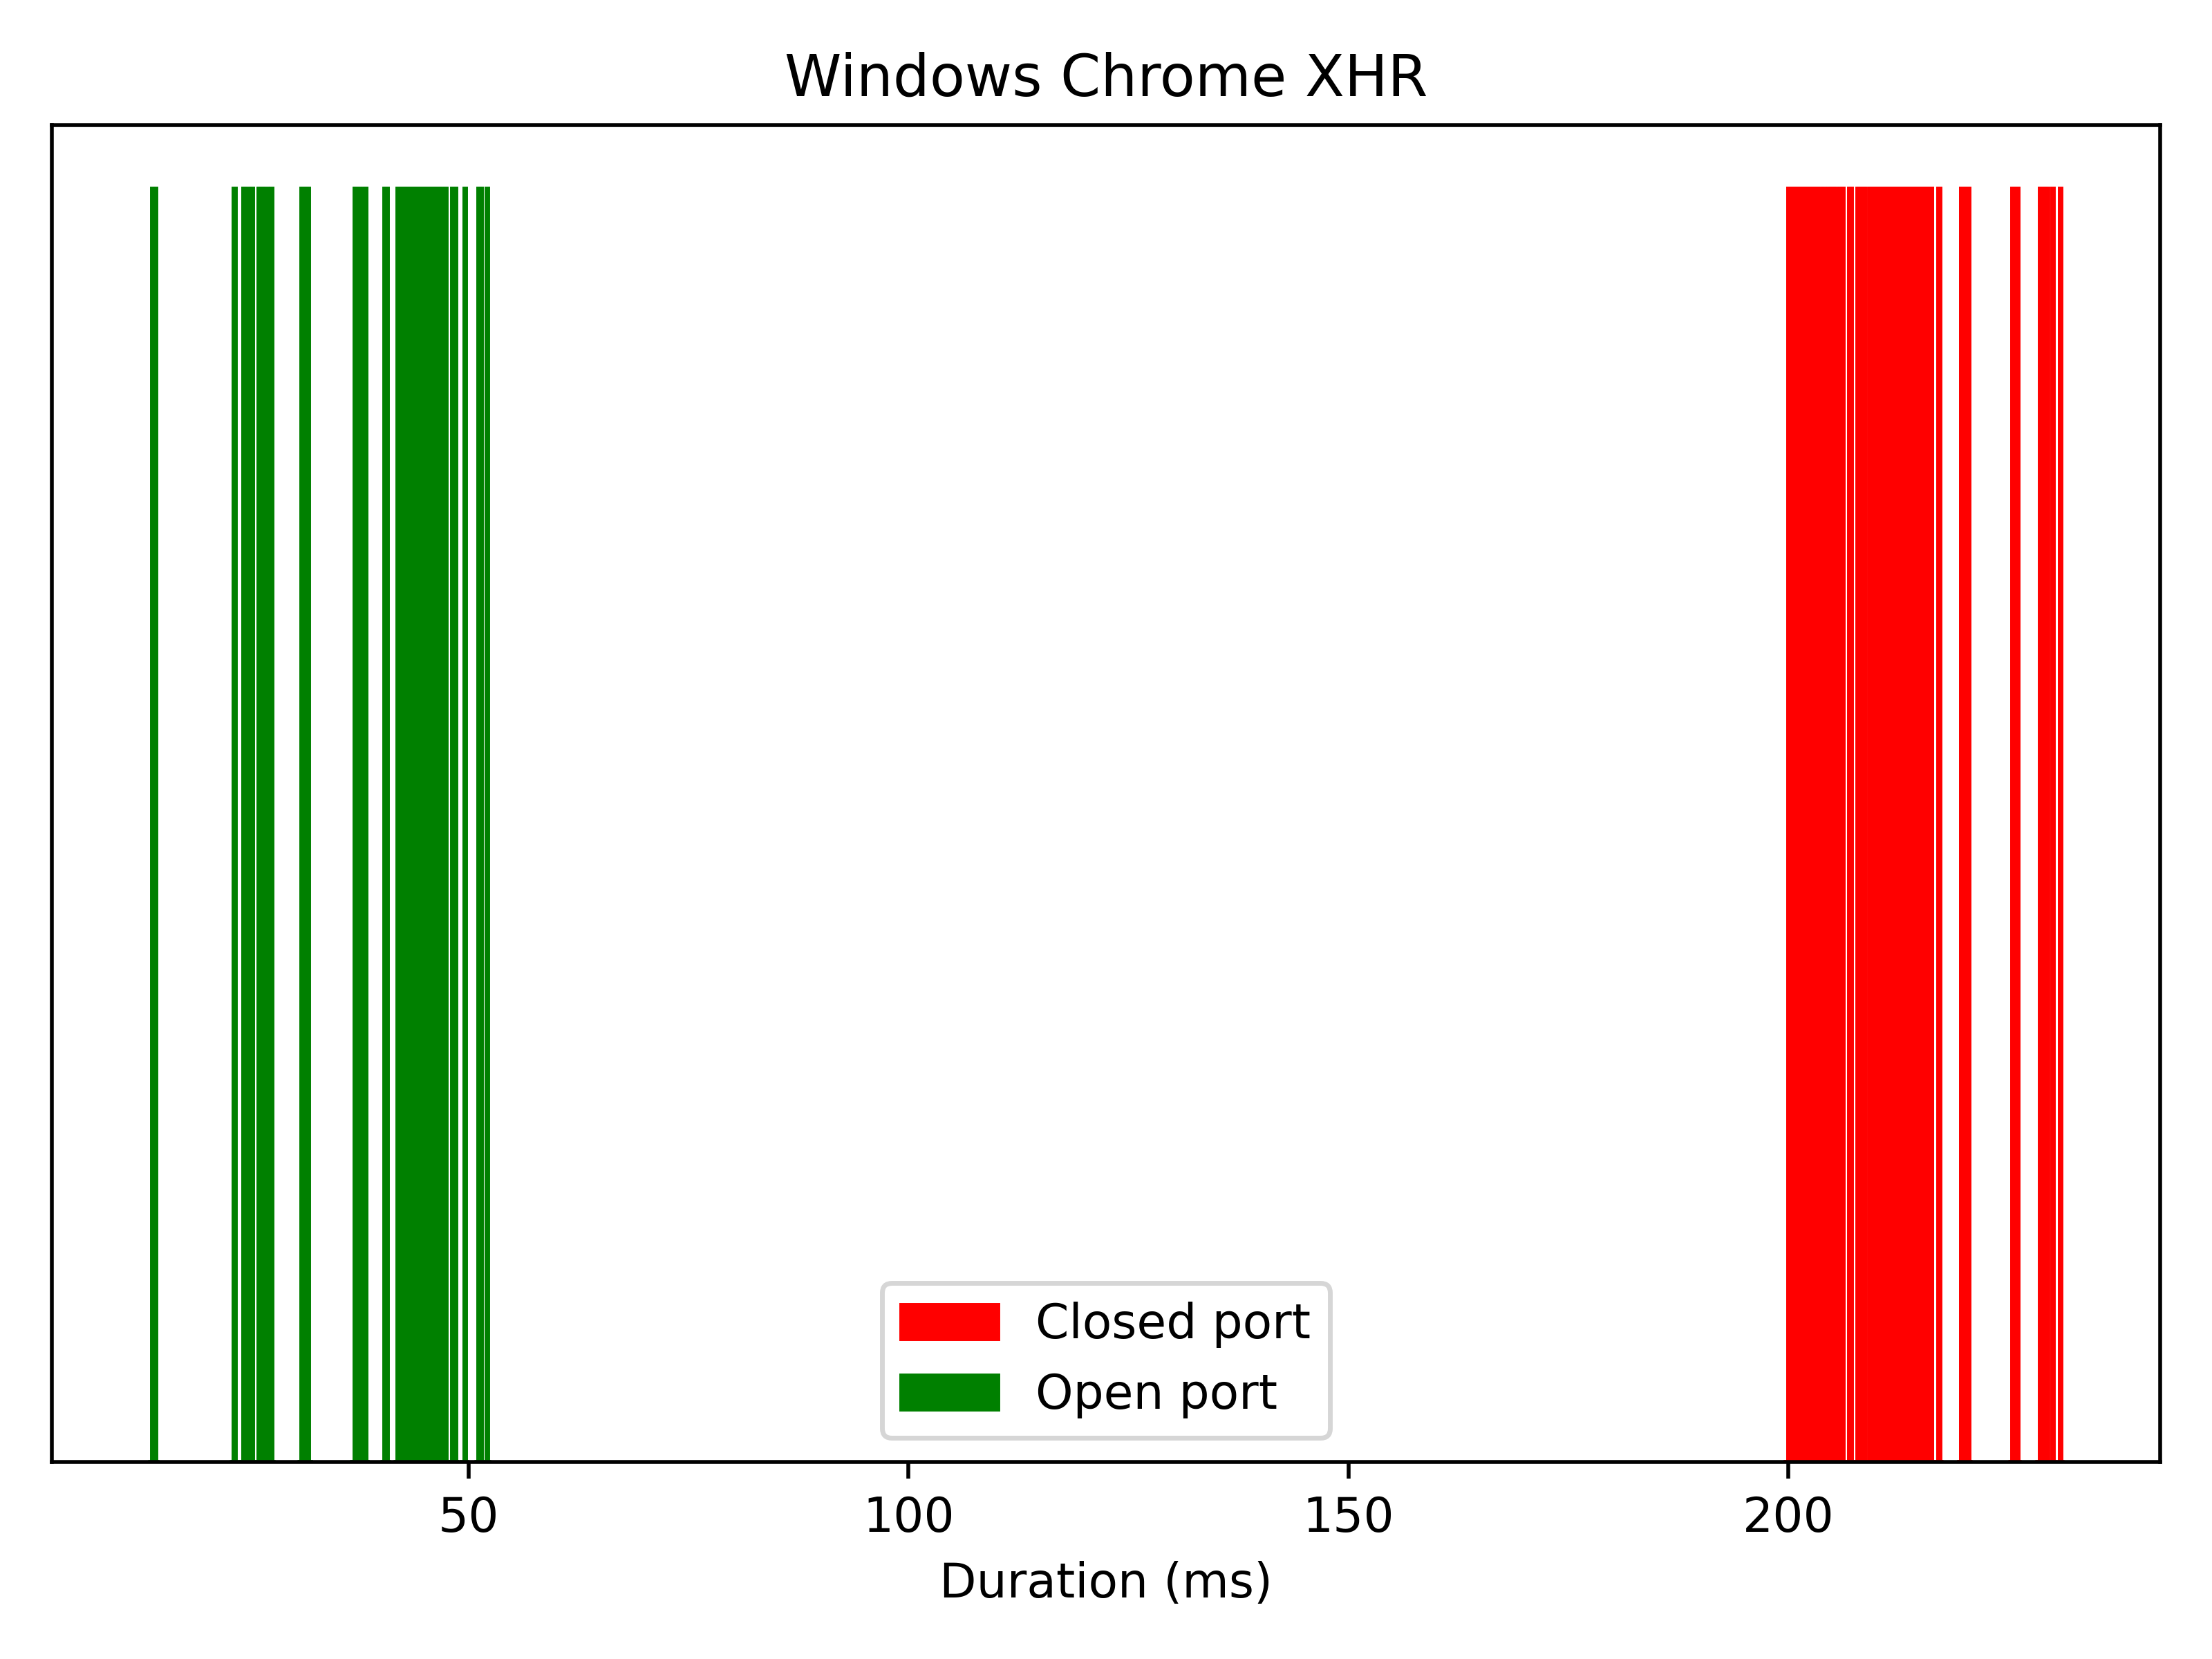
\includegraphics[width=10cm, height=5cm, keepaspectratio]{port_scanning_techniques/img/windows_chrome_efficacy_xhr.png}
%     \caption{Windows/Chrome XHR API scan duration open vs closed ports}
%     \label{fig:win-chrome-xhr}
% \end{minipage}
% \hspace{0.5cm} % Adjust the horizontal space between the two figures
% \begin{minipage}{.45\textwidth}
% \includegraphics[width=10cm, height=5cm, keepaspectratio]{port_scanning_techniques/img/windows_firefox_efficacy_xhr.png}
%     \caption{Windows/Firefox XHR API scan duration open vs closed ports}
%     \label{fig:win-firefox-xhr}
% \end{minipage}
% \end{figure}

% The combination of WebSocket/Firefox also had an increased detection rate of 100\%, but WebSocket/Chrome remained unable to detect any of the open ports, this is depicted in Figures~\ref{fig:win-firefox-websocket} and~\ref{fig:win-chrome-websocket}.

% \begin{figure}[ht]
% \centering
% \begin{minipage}{.45\textwidth}
%   \centering
% \includegraphics[width=8cm, height=4cm, keepaspectratio]{port_scanning_techniques/img/windows_Firefox_efficacy_websocket.png}
%     \caption{Windows/Firefox WebSocket API scan duration open vs closed ports}
%     \label{fig:win-firefox-websocket}
% \end{minipage}
% \hspace{0.5cm} % Adjust the horizontal space between the two figures
% \begin{minipage}{.45\textwidth}
%   \centering
% 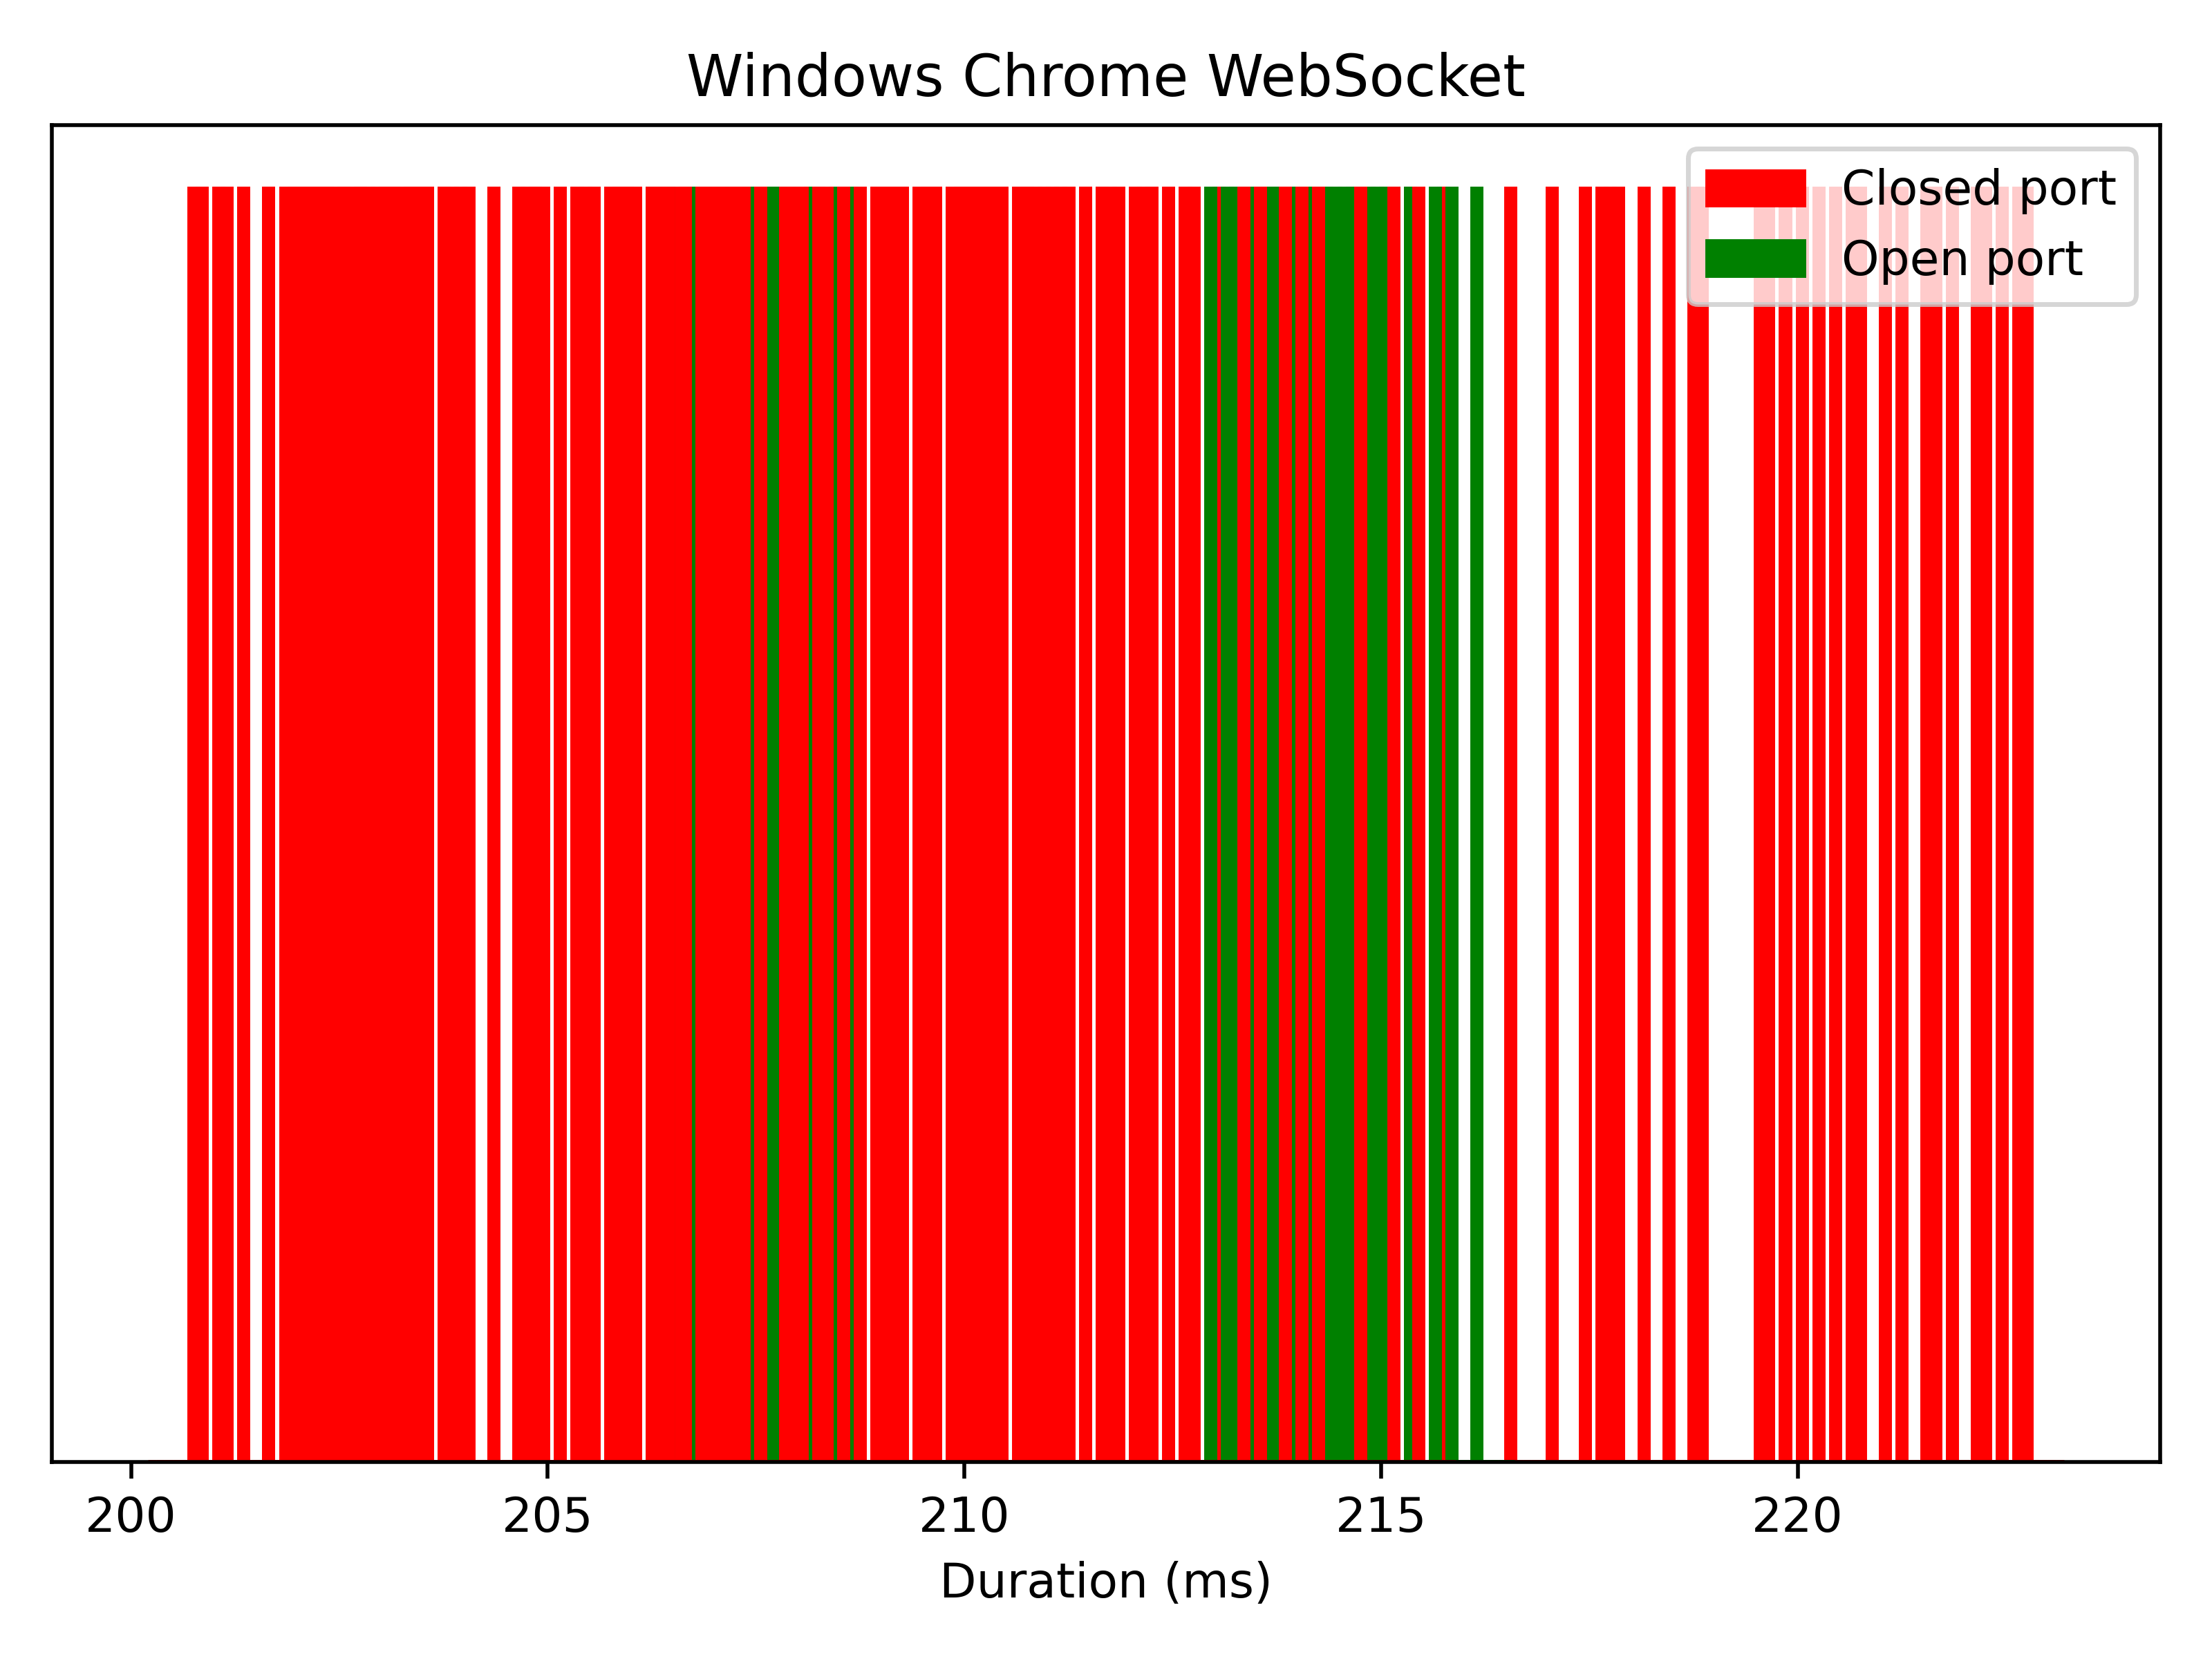
\includegraphics[width=8cm, height=4cm, keepaspectratio]{port_scanning_techniques/img/windows_chrome_efficacy_websocket.png}
%     \caption{Windows/Chrome WebSocket API scan duration open vs closed ports}
%     \label{fig:win-chrome-websocket}
% \end{minipage}
% \end{figure}

% On the contrary, this timing attack method is not useable on the Ubuntu operating system, as there is no clear difference in response times between open and closed ports.

% \subsubsection{Estimating the most efficient scanning technique}

% In this experiment, a comparative analysis of various scanning techniques was conducted to assess their efficiency in scanning the complete port range (0-65536) using different levels of parallel connections. Notable distinctions between Ubuntu and Windows emerged during the utilization of Fetch and XHR APIs, as evidenced in Figures~\ref{fig:windows_chrome_n_sockets} and~\ref{fig:ubuntu_chrome_n_sockets}.

% In the case of Ubuntu, increasing the number of parallel connections does not provide a significant benefit. As soon as roughly 10 parallel connections are used, not much performance gain can be seen when the number of parallel sockets is increased. In fact, performance is slightly decreased with a larger number of parallel connections. 

% Conversely, Ubuntu showed superior performance in scanning individual ports compared to Windows. This discrepancy can be attributed to Ubuntu's disregard for the configured socket timeout of 200ms, a behavior that persisted unless  WebSockets were used. Specifically, under WebSockets usage, Ubuntu's behavior aligned with that of Windows. As a result, the execution of Fetch and XHR connections on Ubuntu occurred notably faster, typically ranging between 5-75ms, in contrast to adhering strictly to the specified 200ms timeout.

% The observed shorter connection timeouts are intrinsically linked to the degree of parallel connections configured. A higher number of parallel connections correlates with an extended timeout duration. Thus, attaining an optimal balance between parallel connections and timeouts proves to be crucial. In this experimental context, the configuration of around 10 parallel connections demonstrated the highest efficiency.

% In conclusion, XHR and Fetch are similar in performance on both Windows and Ubuntu. However, scans complete much faster on Ubuntu than Windows, due to the configured socket timeout not being respected on Ubuntu. WebSockets are similar in performance to XHR and Fetch on Windows, but are significantly outperformed on Ubuntu.  

% \begin{figure}[h]
% \begin{adjustwidth}{-3cm}{-1cm}
% \centering
% \begin{minipage}{.45\textwidth}
%   \centering
% 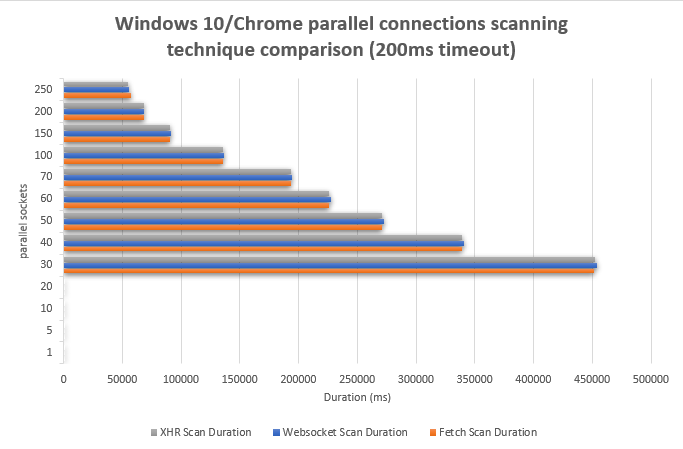
\includegraphics[width=12cm, height=7cm, keepaspectratio]{port_scanning_techniques/img/windows_chrome_scan_technique_comparison.png}
%     \caption{Windows/Chrome Parallel sockets efficiency comparison}
%     \label{fig:windows_chrome_n_sockets}
% \end{minipage}
% \hspace{0.5cm}
% \begin{minipage}{.45\textwidth}
% 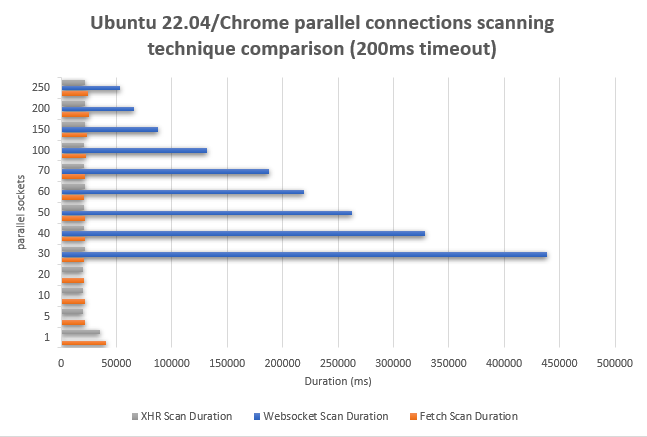
\includegraphics[width=12cm, height=7cm, keepaspectratio]{port_scanning_techniques/img/ubuntu_chrome_scan_technique_comparison.png}
%     \caption{Ubuntu/Chrome Parallel sockets efficiency comparison}
%     \label{fig:ubuntu_chrome_n_sockets}
% \end{minipage}
% \end{adjustwidth}
% \end{figure}


% This optimization on Ubuntu, wherein it disregards the configured socket timeout setting, results in notably faster scans when compared to Windows. 
% Ubuntu completes scanning the entire port range (0-65536) within 25 seconds, whereas Windows takes 50 seconds even with the highest number of parallel connections (250).

% Although using such a high number of parallel connections may seem beneficial in theory, it introduces severe delays and renders the webpage unusable for the user. This consideration underscores the irrelevance of establishing a theoretical limited for parallel connections, such as increasing the count to 256 instead of 250. Both amounts are impractical in real-world scenarios, and a local port scan attack on Windows will not come close to reaching the theoretical limit in practice.




% However, this does not necessarily mean that XHR and WebSockets can not detect open ports. Through post-scan analysis, we can conduct a trivial timing attack~\cite{Dhem2000}, by comparing the response times of the APIs, and comparing the results between open and closed ports. With this methodology, the XHR API can also detect 100\% of open ports, on Windows. 



% \clearpage
% \section{Analysis}

% \subsection{Efficiency}

% There is a clear distinction between Ubuntu and Windows when it comes to running the Fetch and XHR APIs, as can be seen in Figures~\ref{fig:ubuntu_chrome_n_sockets} and~\ref{fig:windows_chrome_n_sockets}. In the case of Ubuntu, increasing the number of parallel connections does not provide a significant benefit. As soon as roughly 10 parallel connections are used, not much performance gain can be seen when the number of parallel sockets is increased. In fact, performance is slightly decreased with a larger number of parallel connections. However, when it comes to scanning individual ports, Ubuntu significantly outperforms Windows. This can be attributed to the fact that Ubuntu ignores the configured socket timeout of 200ms, unless WebSockets are used. In the case of WebSockets, we observe similar behavior to Windows. As a result, Fetch and XHR connections are timed out much faster on Ubuntu, typically within 1-50ms as opposed to the configured 200ms timeout. These timeouts are closely related to the amount of parallel connections. When the number of connections increase, so does the timeout. Striking a balance between parallel connections and timeouts is therefore very important, with the most efficient setting being around 10 parallel connections during our testing. 

% This optimization on Ubuntu leads to significantly faster scans compared to Windows. In just 25 seconds, Ubuntu can scan the entire port range (0-65536), whereas Windows takes 50 seconds even with the highest number of parallel connections (250). Although using such a high number of parallel connections may seem beneficial in theory, it introduces severe delays and renders the webpage unusable for the user. Due to this, determining the theoretical limit for parallel connections, such as 256 connections instead of 250, was considered irrelevant. Both amounts are impractical in real-world scenarios, and a local port scan attack on Windows will not come close to reaching the theoretical limit in practice.

% \subsection{Efficacy}

% As can be seen in appendix A, table~\ref{tab:scan-technique-comparison}, the Fetch API is able to detect 100\% of the open HTTP ports on both Windows and Ubuntu, via the intended functionality of the API. On top of that, both the Fetch and XHR APIs seem to outperform Websockets on both Windows and Ubuntu.

% While it may seem that the XHR API cannot detect any of the open ports, this is not necessarily true. Via post-scan analysis, it is possible to detect the open ports by comparing response times. Open ports respond faster than the configured socket timeout (200ms). Therefore, ports may \emph{generally} be considered open ports when they respond in <200ms. However, \emph{unsafe} ports will respond quickly, but that does not mean that they are open ports. Unsafe or restricted ports refer to a range of TCP/UDP ports that are reserved for system or administrative use and are not meant for normal application traffic. Browsers do not reveal information about these ports, so we cannot determine whether these ports are open or not. Unsafe ports were excluded from the port scans in table~\ref{tab:scan-technique-comparison} to prevent data pollution.

% As can be seen in Figures~\ref{fig:win-chrome-fetch},~\ref{fig:win-chrome-xhr} and~\ref{fig:win-chrome-websocket}, both the XHR and Fetch APIs are able to detect 100\% of open ports through post-scan analysis on Windows. The response times of open ports are significantly faster than closed ports. However, Websockets do not respond faster to open HTTP ports, and can therefore not detect open HTTP ports. As noted before, the configured socket timeout for the scans does not seem to be respected by Ubuntu, this is reflected in figures~\ref{fig:ubuntu-chrome-fetch} and~\ref{fig:ubuntu-chrome-xhr}. Therefore, we cannot rely on response time measurements on Ubuntu. This leaves only the Fetch API as a viable port scanning technique for HTTP webservers on Ubuntu, as opposed to both the Fetch and XHR API on Windows.

% Determining the optimal socket timeout setting is relatively simple. The timeout should be as low as possible while maintaining accuracy. We noticed that a socket timeout of less than 140 milliseconds led to a loss of accuracy on Chrome, resulting in the detection of fewer than 100 open ports. Hence, based on our findings, we conclude that the optimal socket timeout setting for Chrome is roughly 150ms. For Firefox this is less efficient, as we saw a loss of accuracy on 390ms, therefore we conclude that the optimal socket timeout for Firefox is roughly 400ms. 

\section{Experiments Conclusions}

The experiments have resulted in the identification of optimal socket configuration settings for browser-based port scanning. Specifically, it is recommended to utilize a socket timeout of 150ms for Chrome and 400ms for Firefox. For Ubuntu, the most effective number of parallel connections is approximately 10, while on Windows, an increased number of parallel connections, up to 250, is advised. However, due to the associated operational impact on webpage usability, a more practical range of 100-150 parallel connections is recommended for real-world attack scenarios, contingent upon the specific webpage characteristics. 
Among the scanning techniques evaluated, the Fetch API emerges as the optimal choice for browser-based port scanning across both Ubuntu and Windows environments, as well as in browsers such as Chrome and Firefox. The Fetch API exhibits comparable performance to XHR and notably surpasses WebSockets in efficiency. A distinct advantage of the Fetch API lies in its capacity to detect the openness of TCP ports running HTTP services directly, eliminating the necessity for post-scan analysis. This capability is attributed to the utilization of the \emph{no-cors} mode.

When using the optimized scanning configuration, notable speed gains are attainable. For instance, the scanning of 1,000 ports can be achieved within one second using Chrome and within three seconds using Firefox. In broader scans, the entire port range (0 - 65,536) necessitates around 70 seconds for completion on Windows and approximately 25 seconds on Ubuntu. This performance differential stems from Ubuntu's expedited socket timeouts, which diverge from the specified timeout value of 150ms.
In practical applications, port scan attacks typically focus on identifying specific, well-known ports, rather than exhaustively scanning the entire port range. In light of this, browser-based port scanning presents a viable attack vector, capable of scanning more than 1,000 ports per second, thus substantiating its practicality for a real-world attack.


% ~\ref{fig:ubuntu-chrome-websocket}


% \subsubsection{Experiment}

% In order to effectively measure and create the most optimal scanning technique depending on the attack goal, an experiment will be conducted as follows:

% \begin{enumerate}
% \item Open the following ports on the system in different states, representing different attack goals:

% \begin{enumerate}[Port]
% \item 10000: TCP port running HTTP
% \item 10001: TCP port running a WebSocket
% \item 10002: UDP port
% \item 10003: UDS (Unix domain socket) port
% \end{enumerate}

% The expectation is that UDS and UDP ports are undetectable, as client-side JavaScript can only connect to TCP ports. While WebRTC can communicate over UDP sockets, we cannot use WebRTC for port scanning.

% \item Run the port scanner application \cite{bvdl2023} multiple times, using the following steps:
% \begin{itemize}
% \item Enumerate the entire port range (0-65536) using every implemented scanning technique.
% \item Enumerate ports 10000-10003 using every implemented scanning technique.
% \item Rerun the scan by increasing the number of parallel sockets and using the lowest socket timeout possible to achieve the most efficient scanning technique.
% \end{itemize}

% \item Collect the following data for analysis:
% \begin{itemize}
% \item Response time measurements
% \item Identified open ports
% \item Accuracy of the scan results
% \end{itemize}

% This experiment will be conducted on various combinations of browsers and operating systems to determine the most effective scanning technique for each browser/OS.
% \end{enumerate}